%Este archivo no tiene contenido, mas allá de configuraciones y\o definiciones.
%todo el contenido se encuentra en los archivos secundarios que son importados por este.

\documentclass[twoside,a4paper]{article}


%\\\\\\\\\\\\\\\\\\\\\\\\\\\
%Packages en uso

%Idiomas diccionario
\usepackage[english, spanish]{babel}
%\usepackage[english]{babel}

\usepackage[utf8x]{inputenc}
%\usepackage[cp1252]{inputenc} 
%\usepackage[ansinew]{inputenc}
\usepackage{ucs}
\usepackage{lmodern} 



%\usepackage[margin=1cm, paperwidth=21.0cm, paperheight=29.6cm]{geometry}



\usepackage[T1]{fontenc} 
\usepackage{graphicx}
\usepackage{float}
\usepackage{longtable}
%\usepackage{tabu}
%\usepackage{floatflt}
\usepackage{fancyhdr}
\usepackage{hyperref}
%\usepackage{url}
\usepackage{amsfonts}
\usepackage{amssymb}
\usepackage{textcomp}
%\usepackage[symbol]{footmisc}
%\usepackage{pst-circ}
%\usepackage{epsfig}
%\usepackage{xkeyval}
\usepackage{tabularx}
\usepackage{booktabs}



\usepackage[usenames,dvipsnames]{color}


%\usepackage{minted}
\usepackage{latexsym}
\usepackage{colortbl}
%\usepackage{pdfpages}
\usepackage{wrapfig}

%\usepackage{listings}
\usepackage{listingsutf8}
%\usepackage{mips}
\usepackage{appendix}
\usepackage{needspace}
\usepackage{ifplatform}
\usepackage{ifthen}


\usepackage{amsmath}
\usepackage{mathrsfs}





%\usepackage{booktabs}
\usepackage{colortbl}
%\usepackage{tabularx}
%\usepackage{amssymb}



%\\\\\\\\\\\\\\\\\\\\\\\\\\\
% FOR GNUPLOT
%\usepackage{tikz}

%\usepackage[miktex]{gnuplottex}
%\usepackage{gnuplot-lua-tikz}
%\usepackage{mathpazo}
%\\\\\\\\\\\\\\\\\\\\\\\\\\\


%\\\\\\\\\\\\\\\\\\\\\\\\\\\
% FOR FIGURE CAPTION COLORS
\usepackage{caption}
\usepackage[svgnames]{xcolor}

%\\\\\\\\\\\\\\\\\\\\\\\\\\\


%\\\\\\\\\\\\\\\\\\\\\\\\\\\
% FOR CVS FILES
\usepackage{pgfplotstable}
\usepackage{datatool}

%\\\\\\\\\\\\\\\\\\\\\\\\\\\


%\\\\\\\\\\\\\\\\\\\\\\\\\\\
% NUMERIC
%\usepackage[noautolanguage]{numprint}
\usepackage{siunitx}
\usepackage{expl3}
\usepackage{intcalc}
\usepackage{fltpoint}
%\\\\\\\\\\\\\\\\\\\\\\\\\\\


%\\\\\\\\\\\\\\\\\\\\\\\\\\\
% FOR EQUATION CAPTION FORMAT, COLORS AND OTHERS

\usepackage{mathtools}

%\\\\\\\\\\\\\\\\\\\\\\\\\\\


%\\\\\\\\\\\\\\\\\\\\\\\\\\\
% LOOPS
\usepackage{forloop}

%\\\\\\\\\\\\\\\\\\\\\\\\\\\


%\\\\\\\\\\\\\\\\\\\\\\\\\\\
%!!!!!!!!!!!!!!!!!!!!!!!!! DETECCION DE PLATAFORMA !!!!!!!!!!!!!!!!!!!!!!!!!!!!!!!!!
%Permite que sea compilado tanto en windows como en *IX sin cambio alguno.
\newboolean{IsWindows}
\ifwindows
\setboolean{IsWindows}{true}
\else
\setboolean{IsWindows}{false}
\fi
%\\\\\\\\\\\\\\\\\\\\\\\\\\\
%!!!!!!!!!!!!!!!!!!!!!!!!!!!!!!!!!!!!!!!!!!!!!!!!!!!!!!!!!!!!!!!!!!!!!!!!!!!!!!!!!!!!

%\\\\\\\\\\\\\\\\\\\\\\\\\\\
%Idiomas
\hyphenrules{spanish}
%\\\\\\\\\\\\\\\\\\\\\\\\\\\



%\\\\\\\\\\\\\\\\\\\\\\\\\\\
%General
\newcommand{\mailto}[1]{\mbox{\href{mailto:#1}{\textcolor{blue}{#1}}}}
\newcommand{\http}[2]{\mbox{\href{#1}{\textcolor{blue}{#2}}}}
%\\\\\\\\\\\\\\\\\\\\\\\\\\\


%\\\\\\\\\\\\\\\\\\\\\\\\\\\
%Comandos personalizados

\newcommand{\titulo}{Trabajo práctico N\textdegree \hspace{1pt} 1}
\newcommand{\titulolargo}{Raíces de ecuaciones}
\newcommand{\materia}{Análisis numérico I - 75.12/95.04}
\newcommand{\fiuba}{Facultad de Ingeniería - UBA}
\newcommand{\cuatrimestre}{1\textsuperscript{er} cuatrimestre de 2018} %\sptext{do} $2^{do}$


\newcommand{\autorA}{César \textsc{Bordagaray}}
\newcommand{\padronA}{79962}
\newcommand{\mailA}{\mailto{c\_bordagaray@hotmail.com}}
\newcommand{\autorB}{Francisco \textsc{Breghelli}}
\newcommand{\padronB}{94696}
\newcommand{\mailB}{\mailto{franciscobreghelli@hotmail.com}} 
\newcommand{\autorC}{Diego \textsc{Luna}}
\newcommand{\padronC}{75451}
\newcommand{\mailC}{\mailto{diegorluna@gmail.com}}


\newcommand{\docenteA}{Mag. Ing. Miryam \textsc{Sassano}}
\newcommand{\docenteB}{Ing. Ignacio \textsc{Bello}}
\newcommand{\docenteC}{Ing. Matías \textsc{Payva}}
\newcommand{\docenteD}{Lic. Andrés \textsc{Porta}}
\newcommand{\docenteE}{Ing. Ezequiel \textsc{García}}

\newcommand{\thedate}{14 de abril de 2018}


\newcommand{\HRule}{\rule{\linewidth}{0.3mm}}

%\\\\\\\\\\\\\\\\\\\\\\\\\\\


%\\\\\\\\\\\\\\\\\\\\\\\\\\\
%Título,  autor del documento y fecha
\title{\titulo}
\author{\autorC}
\date{\thedate}
%\\\\\\\\\\\\\\\\\\\\\\\\\\\


%\\\\\\\\\\\\\\\\\\\\\\\\\\\
\setcounter{secnumdepth}{5}
\setcounter{tocdepth}{5}
%\\\\\\\\\\\\\\\\\\\\\\\\\\\


%\\\\\\\\\\\\\\\\\\\\\\\\\\\
%suppress widows and orphans
\widowpenalty=9999
\clubpenalty=9999
%\\\\\\\\\\\\\\\\\\\\\\\\\\\


%\\\\\\\\\\\\\\\\\\\\\\\\\\\
%equation numbers to subsection level
%\numberwithin{equation}{subsection}
\numberwithin{equation}{section}
%\\\\\\\\\\\\\\\\\\\\\\\\\\\


%\\\\\\\\\\\\\\\\\\\\\\\\\\\
%equation numbers to subsection level
%\numberwithin{table}{subsection}
\numberwithin{table}{section}
%\\\\\\\\\\\\\\\\\\\\\\\\\\\



%\\\\\\\\\\\\\\\\\\\\\\\\\\\
%figure numbers to subsection level
%\renewcommand{\thefigure}{\thesubsection.\arabic{figure}}
\renewcommand{\thefigure}{\thesection.\arabic{figure}}
%\\\\\\\\\\\\\\\\\\\\\\\\\\\

%\setlength{\arrayrulewidth}{0.6pt}

%\\\\\\\\\\\\\\\\\\\\\\\\\\\
% Highlight equation
\newcommand{\highlight}[2]{\mathchoice%
  {\colorbox{#1}{$\displaystyle#2$}}%
  {\colorbox{#1}{$\textstyle#2$}}%
  {\colorbox{#1}{$\scriptstyle#2$}}%
  {\colorbox{#1}{$\scriptscriptstyle#2$}}}%
%\\\\\\\\\\\\\\\\\\\\\\\\\\\


%\\\\\\\\\\\\\\\\\\\\\\\\\\\
\newcolumntype{z}[1]{%
>{\centering\hspace{0pt}}p{#1}}%

\newcolumntype{y}[1]{%
>{\raggedleft\hspace{0pt}}p{#1}}% 

\newcolumntype{x}[1]{%
>{\raggedright\hspace{0pt}}p{#1}}% 

\newcolumntype{w}[1]{%
>{\centering\hspace{0pt}}m{#1}}%

\newcolumntype{v}[1]{%
>{\raggedleft\hspace{0pt}}m{#1}}% 

\newcolumntype{u}[1]{%
>{\raggedright\hspace{0pt}}m{#1}}% 


\newcommand{\tn}{\tabularnewline}
%\\\\\\\\\\\\\\\\\\\\\\\\\\\




%\\\\\\\\\\\\\\\\\\\\\\\\\\\
% Generales
\newcommand{\quotemarks}[1]{``#1''}
\newcommand{\simplequotemarks}[1]{`#1'}
%\\\\\\\\\\\\\\\\\\\\\\\\\\\


%\\\\\\\\\\\\\\\\\\\\\\\\\\\
% Símbolos de las unidades

\newcommand{\volt}[1]{\mbox{#1 V}}
\newcommand{\milivolt}[1]{\mbox{#1 mV}}
\newcommand{\hertz}[1]{\mbox{#1 Hz}}
\newcommand{\kilohertz}[1]{\mbox{#1 kHz}}
\newcommand{\megahertz}[1]{\mbox{#1 MHz}}
\newcommand{\farad}[1]{\mbox{#1 F}}
\newcommand{\nanofarad}[1]{\mbox{#1 nF}}
\newcommand{\microfarad}[1]{\mbox{#1 $\mu$F}}
\newcommand{\picofarad}[1]{\mbox{#1 pF}}
\newcommand{\fentofarad}[1]{\mbox{#1 fF}}
\newcommand{\ohm}[1]{\mbox{#1 $\Omega$}}
\newcommand{\miliohm}[1]{\mbox{#1 m$\Omega$}}
\newcommand{\kiloohm}[1]{\mbox{#1 k$\Omega$}}
\newcommand{\megaohm}[1]{\mbox{#1 M$\Omega$}}
\newcommand{\amper}[1]{\mbox{#1 A}}
\newcommand{\miliamper}[1]{\mbox{#1 mA}}
\newcommand{\microamper}[1]{\mbox{#1 $\mu$A}}
\newcommand{\picoamper}[1]{\mbox{#1 pA}}
\newcommand{\fentoamper}[1]{\mbox{#1 fA}}
\newcommand{\s}[1]{\mbox{#1 s}}
\newcommand{\milis}[1]{\mbox{#1 ms}}
\newcommand{\micros}[1]{\mbox{#1 $\mu$s}}
\newcommand{\nanos}[1]{\mbox{#1 ns}}
\newcommand{\miliamperporvolt}[1]{ \mbox{#1 $\frac{mA}{V}$}}
\newcommand{\miliamperporvoltcuad}[1]{ \mbox{#1 $\frac{mA}{V^2}$}}
\newcommand{\decibel}[1]{\mbox{#1 dB}}
\newcommand{\decibeli}[1]{\mbox{#1 dBi}}

\newcommand{\spice}{\mbox{\textit{\textbf{SPICE}}}}
\newcommand{\schematic}{\mbox{\textit{\textbf{SCHEMATIC}}}}

% Nombres de las unidades
\newcommand{\Metro}{\mbox{metro}}
\newcommand{\Volt}{\mbox{Volt}}
\newcommand{\Amper}{\mbox{Ampere}}
\newcommand{\Farad}{\mbox{Farad}}
%\\\\\\\\\\\\\\\\\\\\\\\\\\\

%\\\\\\\\\\\\\\\\\\\\\\\\\\\
% Dispositivos

\newcommand{\mosfet}{\mbox{\textbf{MOSFET}}}
\newcommand{\nmosfet}{\mbox{\textbf{NMOSFET}}}
\newcommand{\bjtnpn}{\mbox{\textbf{BJT NPN}}}
\newcommand{\bjtpnp}{\mbox{\textbf{BJT PNP}}}

%\\\\\\\\\\\\\\\\\\\\\\\\\\\

%\\\\\\\\\\\\\\\\\\\\\\\\\\\
% Plataformas

\newcommand{\platformhost}{\textbf{x86(\_64)\textbackslash Linux}}
\newcommand{\platformguest}{\textbf{pmax\textbackslash NetBSD}}

\newcommand{\oshost}{\textbf{Linux}}
\newcommand{\osguest}{\textbf{NetBSD}}

\newcommand{\MIPS}{\textbf{MIPS32}}
%\\\\\\\\\\\\\\\\\\\\\\\\\\\


%\\\\\\\\\\\\\\\\\\\\\\\\\\\
% Programación

\newcommand{\GNU}{\textbf{GNU}}

\newcommand{\GCC}{\textbf{GCC}}

\newcommand{\GDB}{\textbf{GDB}}

\newcommand{\GXEMUL}{\textbf{GXemul}}

\newcommand{\langc}{\textbf{\quotemarks{C}}}

\newcommand{\langass}{\textbf{assembly}}

\newcommand{\langmipsass}{\textbf{MIPS32 assembly}}

\newcommand{\make}{\textbf{make}}
%\\\\\\\\\\\\\\\\\\\\\\\\\\\


%\\\\\\\\\\\\\\\\\\\\\\\\\\\
% Archivos

\newcommand{\quotefile}[1]{\textit{\quotemarks{#1}}}

\newcommand{\filebox}[2]{%

\begin{tabular}{l}

\multicolumn{1}{>{\columncolor{#2}}l}{#1} 
	
\end{tabular}

}%
%\\\\\\\\\\\\\\\\\\\\\\\\\\\



%\\\\\\\\\\\\\\\\\\\\\\\\\\\
% Math
\newcommand{\Reales}{\mathbb{R}}
\newcommand{\Complejos}{\mathbb{C}}
\newcommand{\numnorm}[1]{\left|#1\right|}
\newcommand{\vectornorm}[1]{\left|\left|#1\right|\right|}
%\\\\\\\\\\\\\\\\\\\\\\\\\\\


%\\\\\\\\\\\\\\\\\\\\\\\\\\\
% Counters
\newcommand{\resetallcounters}{%
\setcounter{figure}{0}
\setcounter{equation}{0}
\setcounter{table}{0}
}%
%\\\\\\\\\\\\\\\\\\\\\\\\\\\



%\\\\\\\\\\\\\\\\\\\\\\\\\\\
% Definiciones de colores.
\definecolor{Deepblue}{rgb}{0.00,0.00,0.70}
\definecolor{Deepgreen}{rgb}{0.09,0.45,0.20}
\definecolor{Darkgreen}{RGB}{0, 128, 0}
\definecolor{Lightgreen}{RGB}{72, 244, 66}
\definecolor{Purple}{rgb}{1,0,1}
\definecolor{Deeppurple}{rgb}{0.2,0,1}
\definecolor{Gray}{rgb}{0.3,0.3,0.3}
\definecolor{Lightblue}{rgb}{0.60, 0.80, 1.00}
\definecolor{Lightblue2}{RGB}{200, 255, 255}
\definecolor{Lightyellow}{rgb}{1.00,1.00,0.60}
\definecolor{LightButter}{rgb}{0.98,0.91,0.31}
\definecolor{LightOrange}{RGB}{244, 182, 66}
\definecolor{LightChocolate}{rgb}{0.91,0.72,0.43}
\definecolor{LightChameleon}{rgb}{0.54,0.88,0.20}
\definecolor{LightSkyBlue}{rgb}{0.45,0.62,0.81}
\definecolor{LightPlum}{rgb}{0.68,0.50,0.66}
\definecolor{LightScarletRed}{rgb}{0.93,0.16,0.16}
\definecolor{Butter}{rgb}{0.93,0.86,0.25}
\definecolor{Orange}{rgb}{0.96,0.47,0.00}
\definecolor{Chocolate}{rgb}{0.75,0.49,0.07}
\definecolor{Chameleon}{rgb}{0.45,0.82,0.09}
\definecolor{SkyBlue}{rgb}{0.20,0.39,0.64}
\definecolor{Plum}{rgb}{0.46,0.31,0.48}
\definecolor{ScarletRed}{rgb}{0.80,0.00,0.00}
\definecolor{DarkButter}{rgb}{0.77,0.62,0.00}
\definecolor{DarkOrange}{rgb}{0.80,0.36,0.00}
\definecolor{DarkChocolate}{rgb}{0.56,0.35,0.01}
\definecolor{DarkChameleon}{rgb}{0.30,0.60,0.02}
\definecolor{DarkSkyBlue}{rgb}{0.12,0.29,0.53}
\definecolor{DarkPlum}{rgb}{0.36,0.21,0.40}
\definecolor{DarkScarletRed}{rgb}{0.64,0.00,0.00}
\definecolor{Aluminium1}{rgb}{0.93,0.93,0.92}
\definecolor{Aluminium2}{rgb}{0.82,0.84,0.81}
\definecolor{Aluminium3}{rgb}{0.73,0.74,0.71}
\definecolor{Aluminium4}{rgb}{0.53,0.54,0.52}
\definecolor{Aluminium5}{rgb}{0.33,0.34,0.32}
\definecolor{Aluminium6}{rgb}{0.18,0.20,0.21}


\definecolor{MATLABKeyword}{RGB}{0,0,255}
\definecolor{MATLABString}{RGB}{160,32,240}
\definecolor{MATLABComment}{RGB}{34,139,34}


\definecolor{EQColor}{rgb}{0.80,0.36,0.00}
\definecolor{FIGColor}{cmyk}{1,0.00,0.00,0.00}
\definecolor{TABLEColor}{RGB}{199,199,0}
\definecolor{FILENAMEFOOTER}{RGB}{250,0,0}


\definecolor{APENDLINKColor}{rgb}{0.96,0.47,0.00}
\definecolor{SECTLINKColor}{rgb}{1.00,0.00,0.00}
\definecolor{FILELINKColor}{rgb}{1.00,0.00,0.00}
\definecolor{INTERNALLINKColor}{rgb}{1.00,0.00,0.00}
\definecolor{WEBLINKColor}{rgb}{0.00,0.00,1.00}
\definecolor{CITELINKColor}{RGB}{141,199,126}
\definecolor{TABLELINKColor}{RGB}{199,199,0}





%\\\\\\\\\\\\\\\\\\\\\\\\\\\


%\\\\\\\\\\\\\\\\\\\\\\\\\\\
% FOR FIGURE CAPTION COLORS

\DeclareCaptionFont{FIGFont}{\color{FIGColor}}
\captionsetup[figure]{labelfont={FIGFont,bf}}

\newcommand{\figref}[1]{\textcolor{FIGColor}{\ref{#1}}}
%\\\\\\\\\\\\\\\\\\\\\\\\\\\


%\\\\\\\\\\\\\\\\\\\\\\\\\\\
% FOR TABLE CAPTION COLORS

\DeclareCaptionFont{TABLEFont}{\color{TABLEColor}}
\captionsetup[table]{labelfont={TABLEFont,bf}}

\newcommand{\tableref}[1]{\textcolor{TABLEColor}{\ref{#1}}}


%\captionsetup[table]{style=fortables}
%\captionsetup[figure]{style=forfigures}
%\\\\\\\\\\\\\\\\\\\\\\\\\\\


%\\\\\\\\\\\\\\\\\\\\\\\\\\\
% FOR EQUATION CAPTION FORMAT, COLORS AND OTHERS

\newtagform{brackets2}[\textcolor{EQColor}]{\textcolor{EQColor}(}{\textcolor{EQColor})}
\usetagform{brackets2}

%\\\\\\\\\\\\\\\\\\\\\\\\\\\


%\\\\\\\\\\\\\\\\\\\\\\\\\\\
% FOR EQUATION CAPTION COLORS
%\makeatletter %% Without ams
%\def\@eqnnum{{\normalfont\normalcolor[\theequation]}}
%\makeatother

%But amsmath redefines the numbering of equations, so then you can do:

%\makeatletter %% With ams
%\def\tagform@#1{\maketag@@@{[\ignorespaces#1\unskip\@@italiccorr]}}
%\makeatother 
%\\\\\\\\\\\\\\\\\\\\\\\\\\\


%\\\\\\\\\\\\\\\\\\\\\\\\\\\
% FOR APENDIX REFERENCE

\newcommand{\apendref}[1]{\textcolor{APENDLINKColor}{\ref{#1}}}

%\\\\\\\\\\\\\\\\\\\\\\\\\\\


%\\\\\\\\\\\\\\\\\\\\\\\\\\\
% FOR SECTION REFERENCE

\newcommand{\sectref}[1]{\textcolor{SECTLINKColor}{\ref{#1}}}

%\\\\\\\\\\\\\\\\\\\\\\\\\\\


%\\\\\\\\\\\\\\\\\\\\\\\\\\\
% WEB LINK

\newcommand{\weblink}[2]{\href{#1}{\textcolor{WEBLINKColor}{#2}}}

%\\\\\\\\\\\\\\\\\\\\\\\\\\\


%\\\\\\\\\\\\\\\\\\\\\\\\\\\
% FILE LINK

\newcommand{\filelink}[2]{\href{#1}{\textcolor{FILELINKColor}{#2}}}

%\\\\\\\\\\\\\\\\\\\\\\\\\\\


%\\\\\\\\\\\\\\\\\\\\\\\\\\\
% CITE LINK
\newcommand{\citelink}[1]{\textcolor{LimeGreen}{\cite{#1}}}

%\\\\\\\\\\\\\\\\\\\\\\\\\\\


\hypersetup{
%	bookmarksnumbered,
%	pdfpagemode={UseOutlines},
%    bookmarks=true,         				% show bookmarks bar?
    unicode=true,          					% non-Latin characters in Acrobat’s bookmarks
    pdftoolbar=true,        				% show Acrobat’s toolbar?
    pdfmenubar=true,        				% show Acrobat’s menu?
%    pdffitwindow=false,    				% window fit to page when opened
%    pdfstartview={FitH},   				% fits the width of the page to the window
    pdftitle={\titulo},   					% title
    pdfauthor={\autorC},    				% author
    pdfsubject={\materia},   				% subject of the document
%    pdfcreator={\LaTeX},   				% creator of the document
%    pdfproducer={Producer},				% producer of the document
    pdfkeywords={TL} {TP}, 					% list of keywords
    pdfnewwindow=true,      				% links in new window
    linktoc=all,							%
    colorlinks=false,  						% false: boxed links; true: colored links	
	linkcolor=INTERNALLINKColor,			% color of internal links
    citecolor=CITELINKColor,    			% color of links to bibliography
    filecolor=FILELINKColor,   	 			% color of file links
    urlcolor=WEBLINKColor,       			% color of external links	
	linkbordercolor=INTERNALLINKColor,		% color of internal links
	citebordercolor=CITELINKColor,			% color of links to bibliography
    filebordercolor=FILELINKColor,    		% color of file links
    urlbordercolor=WEBLINKColor}	       	% color of external links	    
   				
	


%\\\\\\\\\\\\\\\\\\\\\\\\\\\
%Comportamiento de los links a archivos externos.
%\hypersetup{pdfnewwindow=true}
%\\\\\\\\\\\\\\\\\\\\\\\\\\\

%\\\\\\\\\\\\\\\\\\\\\\\\\\\
%Tamaños de la página y margenes

\linespread{1.3}
\oddsidemargin .1cm
\evensidemargin .1cm
\textwidth 16.5cm
\topmargin 0in
\voffset = 0pt
\textheight 21.08cm %8.3in
%\\\\\\\\\\\\\\\\\\\\\\\\\\\



%\pagestyle{fancy}


%\\\\\\\\\\\\\\\\\\\\\\\\\\\
%Encabezado y pie de páginas para todas las páginas normales

\fancypagestyle{allpages}{%

\fancyhf{}  

\renewcommand{\headrulewidth}{0.4pt}
\renewcommand{\footrulewidth}{0.4pt}

%No convierte a mayúscula los nombres de capítulo y sección 
%ni muestra el número.
%\renewcommand{\chaptermark}[1]{}
\renewcommand{\sectionmark}[1]{\markright{##1}{}}
\renewcommand{\subsectionmark}[1]{}
\renewcommand{\subsubsectionmark}[1]{}


\setlength{\headheight}{12pt}

   
%\fancyhf[LOH,REH]{\fiuba}
%\fancyhf[ROH,LEH]{\titulo}

\fancyhf[LH]{\small{\fiuba}}
\fancyhf[CH]{\small{\materia}}
\fancyhf[RH]{\titulo} 

\fancyhf[LOF,REF]{\small{\cuatrimestre}}
\fancyhf[CF]{\small{\rightmark}}
\fancyhf[LEF, ROF]{\textbf{\thepage}} 

}

%\\\\\\\\\\\\\\\\\\\\\\\\\\\


%\\\\\\\\\\\\\\\\\\\\\\\\\\\
%Encabezado y pie de páginas para el índice
\fancypagestyle{indexstyle}{%

\fancyhf{} % clear all header and footer fields

\renewcommand{\headrulewidth}{0.4pt}
\renewcommand{\footrulewidth}{0.4pt}

\setlength{\headheight}{12pt}


\fancyhf[LH]{\small{\fiuba}}
\fancyhf[CH]{\small{\materia}}
\fancyhf[RH]{\titulo}

\fancyhf[LOF,REF]{\small{\cuatrimestre}}
\fancyhf[CF]{\small{Índice}}
\fancyhf[LEF, ROF]{\textbf{\thepage}} 

%\color{red}

}
%\\\\\\\\\\\\\\\\\\\\\\\\\\\




%\\\\\\\\\\\\\\\\\\\\\\\\\\\
%Encabezado y pie de páginas para el código
\fancypagestyle{codestyle}{%

\fancyhf{} % clear all header and footer fields

\renewcommand{\headrulewidth}{0.4pt}
\renewcommand{\footrulewidth}{0.4pt}

%No convierte a mayúscula los nombres de capítulo y sección 
%ni muestra el número.
%\renewcommand{\chaptermark}[1]{}
\renewcommand{\sectionmark}[1]{}
\renewcommand{\subsectionmark}[1]{}
\renewcommand{\subsubsectionmark}[1]{\markright{##1}}

\setlength{\headheight}{12pt}

\fancyhf[LH]{\small{\fiuba}}
\fancyhf[CH]{\small{\materia}}
\fancyhf[RH]{\titulo}
\fancyhf[LOF,REF]{\small{\cuatrimestre}}
\fancyhf[CF]{\small{Archivo: \color{FILENAMEFOOTER}\rightmark}}
%\bfseries{\color{red} \filename
\fancyhf[LEF, ROF]{\textbf{\thepage}} 


\normalfont
}
%\\\\\\\\\\\\\\\\\\\\\\\\\\\



\newcommand{\themark}{}

%\\\\\\\\\\\\\\\\\\\\\\\\\\\
%Encabezado y pie de páginas para el código
\fancypagestyle{codeconsstyle}{%

\fancyhf{} % clear all header and footer fields

\renewcommand{\headrulewidth}{0.4pt}
\renewcommand{\footrulewidth}{0.4pt}


\setlength{\headheight}{12pt}


\fancyhf[LH]{\small{\fiuba}}
\fancyhf[CH]{\small{\materia}}
\fancyhf[RH]{\titulo}

\fancyhf[LOF,REF]{\small{\cuatrimestre}}
\fancyhf[CF]{\small{\themark}}
\fancyhf[LEF, ROF]{\textbf{\thepage}} 

}
%\\\\\\\\\\\\\\\\\\\\\\\\\\\




%\\\\\\\\\\\\\\\\\\\\\\\\\\\
%Encabezado y pie de páginas para el índice
\fancypagestyle{bibliostyle}{%

\fancyhf{} % clear all header and footer fields

\renewcommand{\headrulewidth}{0.4pt}
\renewcommand{\footrulewidth}{0.4pt}

\setlength{\headheight}{12pt}


\fancyhf[LH]{\small{\fiuba}}
\fancyhf[CH]{\small{\materia}}
\fancyhf[RH]{\titulo}

\fancyhf[LOF,REF]{\small{\cuatrimestre}}
\fancyhf[CF]{\small{Bibliografía}}
\fancyhf[LEF, ROF]{\textbf{\thepage}} 

}
%\\\\\\\\\\\\\\\\\\\\\\\\\\\



%\\\\\\\\\\\\\\\\\\\\\\\\\\\
%Renuevo los nombres de los apéndices.
\renewcommand{\appendixpagename}{Apéndices}
\renewcommand{\appendixtocname}{Apéndices}
%\\\\\\\\\\\\\\\\\\\\\\\\\\\

%\\\\\\\\\\\\\\\\\\\\\\\\\\\
%Renuevo el símbolo de los items.
\renewcommand\labelitemi{$\bullet$}
%\\\\\\\\\\\\\\\\\\\\\\\\\\\


%\\\\\\\\\\\\\\\\\\\\\\\\\\\
%Uso el punto decimal en lugar de la coma aunque este en español.
\decimalpoint
%\\\\\\\\\\\\\\\\\\\\\\\\\\\


%\\\\\\\\\\\\\\\\\\\\\\\\\\\\\\\

%-------------------------------------------------
%--------------- BEGIN DOCUMENT ------------------
%-------------------------------------------------
\begin{document}



%\\\\\\\\\\\\\\\\\\\\\\\\\\\
%Incluyo la caratula
%Caratula
\begin{titlepage}
%
% Sin cabecera ni pie de página:
%


\thispagestyle{empty}


 %Título:

	\begin{center}

   	\begin{figure}[H]
    		\centering
    		
\includegraphics[width=0.7 \textwidth]{./img/fiuba}
  	\end{figure}




		\vspace{2.0cm}


		\textsc{\huge \materia}\\
		\vspace{1cm}
		\Huge{\titulo}\\
		\HRule \\
		\vspace{0.4cm}
		\Large{\textbf{\titulolargo}}\\
		\HRule \\
		\vspace{0.4cm}



		\begin{flushleft}
			\begin{tabularx}{\textwidth}{@{\extracolsep{\fill}} ll|l}
				\emph{Alumnos:}&&\emph{Docentes:} \\
				\autorA & Padrón N\textdegree \space \padronA & \docenteA \\
				\mailA &&\docenteB \\
				\autorB & Padrón N\textdegree \space \padronB & \docenteC\\
				\mailB &&\docenteD\\		
				\autorC & Padrón N\textdegree \space \padronC & \docenteE\\
				\mailC && \\	
				\autorD & Padrón N\textdegree \space \padronD & \docenteF\\
				\mailD && \\								
				&&\\
				%&&\begin{normalsize}\textbf{(*) Docente asignado.}\end{normalsize}\\				
			\end{tabularx}
		\end{flushleft}

		%\vspace{0.6cm}


		\vfill

		% Bottom of the page
		{\Large \thedate}

	\end{center}


\end{titlepage}














\thispagestyle{empty}
\cleardoublepage
%\\\\\\\\\\\\\\\\\\\\\\\\\\\
	
%\\\\\\\\\\\\\\\\\\\\\\\\\\\
%Reinicio la cuenta y seteo el estilo de headers y footers.
\pagestyle{indexstyle}
\pagenumbering{Roman}
\setcounter{page}{1}
%\\\\\\\\\\\\\\\\\\\\\\\\\\\

%\\\\\\\\\\\\\\\\\\\\\\\\\\\
\begin{small}
\pagestyle{indexstyle}
\pagenumbering{Roman}

\tableofcontents 
\addcontentsline{toc}{section}{Índice}

%\phantomsection\pdfbookmark[0]{\indexname}{bookmarkForTheIndex}

\cleardoublepage

\pagestyle{indexstyle}
\pagenumbering{Roman}

\listoffigures
\addcontentsline{toc}{section}{Índice de figuras}

\pagestyle{indexstyle}
\pagenumbering{Roman}

\cleardoublepage

\pagestyle{indexstyle}
\pagenumbering{Roman}

\listoftables
\addcontentsline{toc}{section}{Índice de cuadros}

\pagestyle{indexstyle}
\pagenumbering{Roman}

\end{small}

\cleardoublepage
%\\\\\\\\\\\\\\\\\\\\\\\\\\\

%\\\\\\\\\\\\\\\\\\\\\\\\\\\
%Reinicio la cuenta y seteo el estilo de headers y footers.
\pagestyle{allpages}
\setcounter{page}{1}
\pagenumbering{arabic}
%\\\\\\\\\\\\\\\\\\\\\\\\\\\

%\\\\\\\\\\\\\\\\\\\\\\\\\\\
\section{Enunciado}
\resetallcounters

\subsection{Resumen enunciado}


%\bfseries{\color{red} Enunciado:}

\normalfont

Este TP consiste en realizar un pequeño estudio del movimiento de un ascensor, figura~\figref{fig:fig_elevator}, intentando utilizar valores realistas para los parámetros a fin de obtener las expresiones para la posición, $x_{(t)}$, la velocidad, $v_{(t)}$ y la aceleración, $a_{(t)}$. Luego estas expresiones se utilizarán para aplicar un método numérico de nuestra implementación, Newton-Raphson en este caso.





\subsection{Planteo}

El planteo implica asumir ciertas cosas acerca del ascensor, realizando el análisis para el movimiento ascendente, en particular se debe analizar, la altura de un piso, que asumimos ser igual para todos los pisos, siendo en todos por lo tanto el mismo problema, la masa de la cabina y los pasajeros, el tiempo de viaje máximo (se da a máxima carga), la máxima aceleración, y la máxima velocidad, asumimos también por simplicidad que la fuerza que se imprime a la cabina varía linealmente con el tiempo, esto es planteado así en el enunciado. Todas estos parámetros se obtuvieron de normas locales,\citelink{camaradeascensores}, e internacionales, \citelink{elevatorworld}, y de algunos ejemplos de ascensores residenciales comerciales.



%%\begin{figure}[!h] %htb
\begin{wrapfigure}{r}{0.5 \linewidth}
\begin{center}
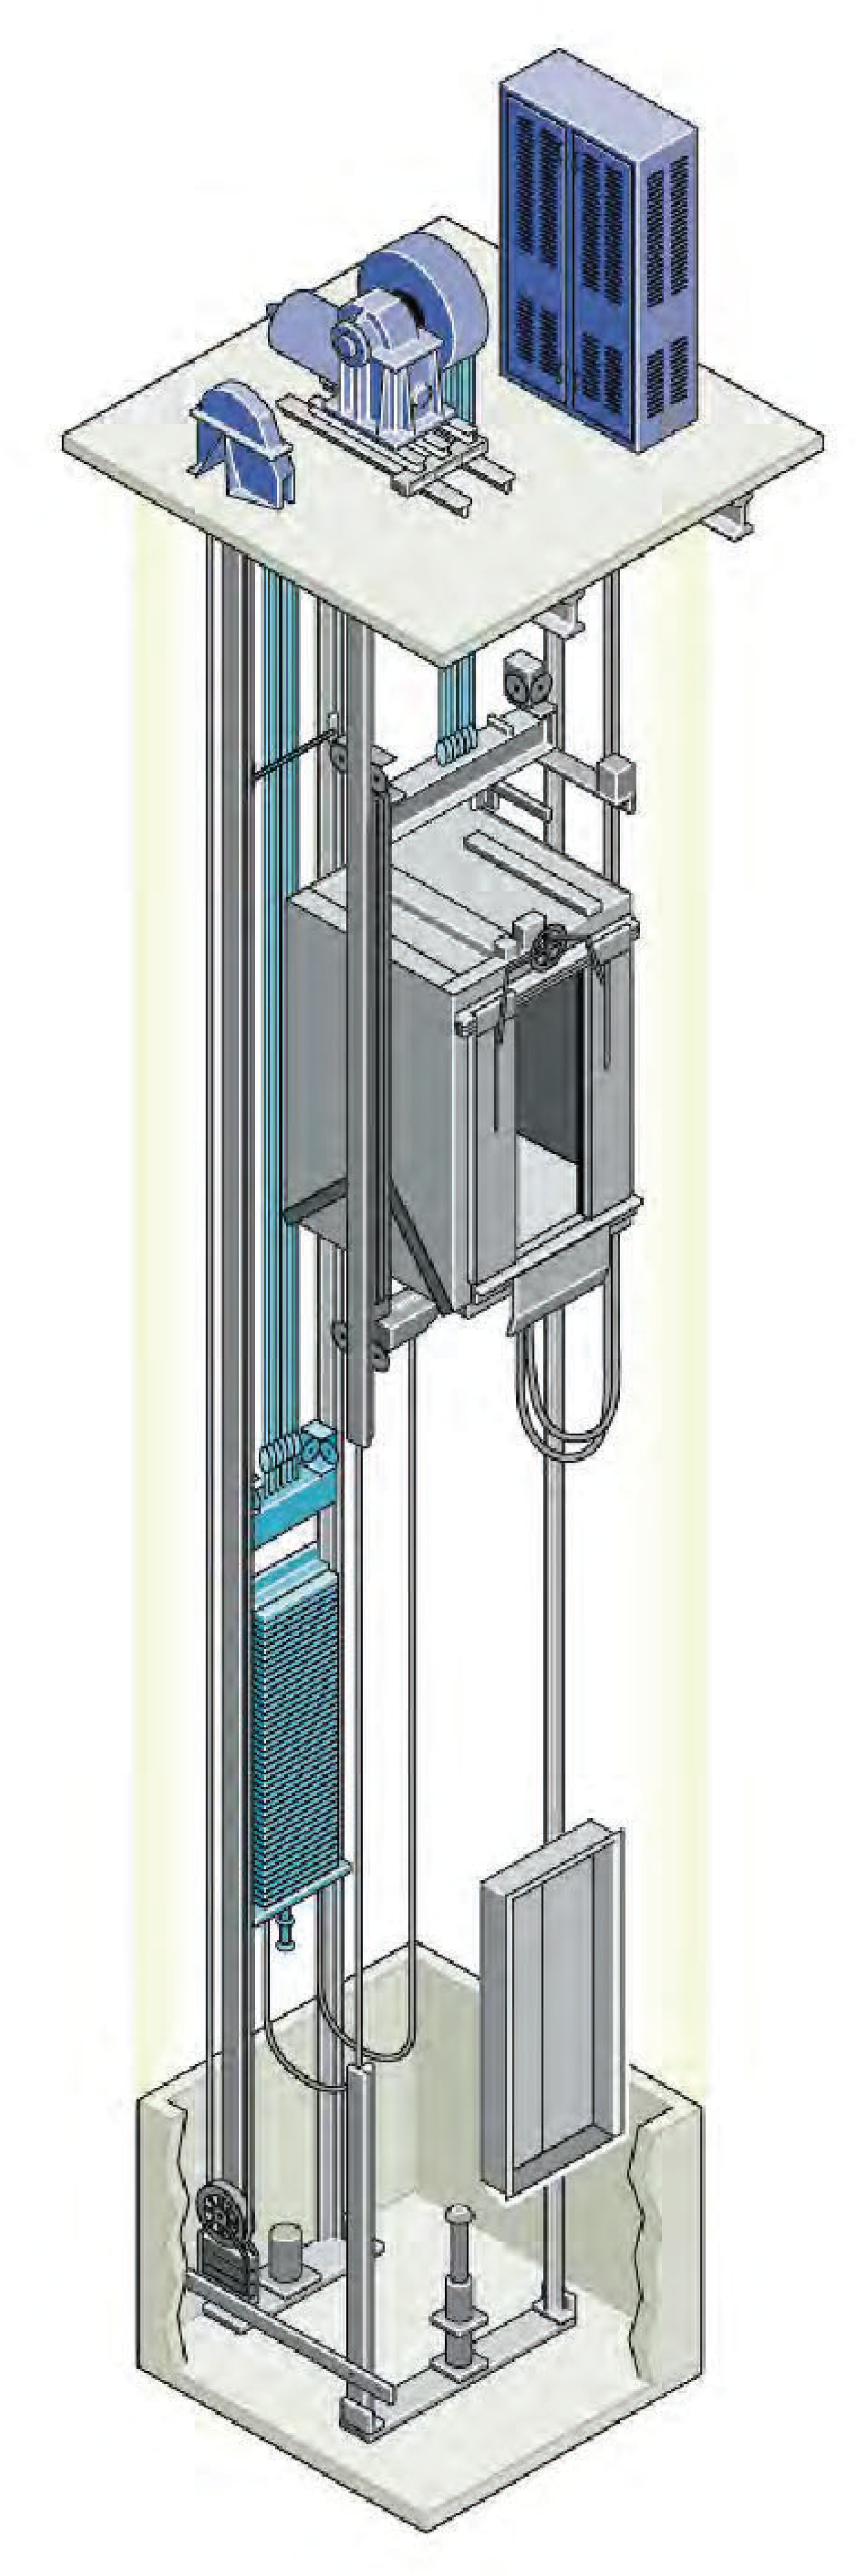
\includegraphics[width=0.35 \linewidth, keepaspectratio=true]{img/diagrams/elevator.png} %% , angle=90 trim={<left> <lower> <right> <upper>}
\caption{\label{fig:fig_elevator} \footnotesize{Ascensor electromecánico.}}
\end{center}
\end{wrapfigure}
%%\end{figure}

En general las normas especifican para la máxima aceleración posible $8 \si[per-mode=symbol]{\meter\per\second\squared}$, la masa de cada persona debe tomarse en promedio como de $75 \si[per-mode=symbol]{\kilogram}$, la masa de la cabina depende del ascensor en cuestión, se tomó un modelo para $12$ personas, con una cabina de masa igual a $450 \si[per-mode=symbol]{\kilogram}$, esto determina la masa máxima de carga en $1350 \si[per-mode=symbol]{\kilogram}$ y la mínima en los $450 \si[per-mode=symbol]{\kilogram}$ de la cabina vacía.


\begin{equation}
x_{(t)} = A \cdot t^{3} + B \cdot t^{2} + C \cdot t + D
\end{equation}

\begin{equation}
v_{(t)} = 3 \cdot A \cdot t^{2} + 2 \cdot B \cdot t + C
\end{equation}

\begin{equation}
a_{(t)} = 6 \cdot A \cdot t + 2 \cdot B \cdot
\end{equation}


\clearpage


\subsection{Resolución}

Para la resolución de la parte de programación del trabajo práctico e implementar los algoritmos pedidos, decidimos usar \textbf{MATLAB}, mayormente por conocerlo previamente y la sencillez con la que se pueden escribir scripts que implementen los algoritmos. A pesar de que la resolución se realizó en \textbf{MATLAB}, se prestó atención a la compatibilidad con \textbf{Octave}, ya que la compatibilidad en los paquetes básicos es alta y con un poco de cuidado y algo de programación condicional se puede lograr que los scripts funcionen en ambos entornos.
Todas las salidas numéricas se guardaron en archivos que luego fueron leídas en \LaTeX\space usando paquetes para el proceso de archivos en formato \textbf{\quotemarks{CSV}}, los mismos permiten redondeo, presentación y hasta algunas operaciones sobre los datos, lo cual facilita el escribir el informe de tal manera de que no deba modificarse al modificar los datos, basta con compilar nuevamente. Las imágenes en forma similar, se guardaron por código desde \textbf{MATLAB} en formato \textbf{\quotemarks{PNG}} y luego se incorporaron desde \LaTeX. Algo a mencionar es que se estimaron lo valores del orden de convergencia y la constante asintótica, para cada uno de los método numéricos implementados, para lograr una buena precisión en las estimaciones se agregó una tolerancia mas a las ya pedidas en el trabajo práctico.



%\cleardoublepage
\clearpage
%\\\\\\\\\\\\\\\\\\\\\\\\\\\

%\\\\\\\\\\\\\\\\\\\\\\\\\\\
\section{Implementación de los algoritmos}
\resetallcounters

El script resuelve en principio los casos pedidos en el enunciado, y luego toma interactivamente con diálogos nuevos parámetros al usuario, los cuales valida y utiliza para resolver el nuevo sistema, en cada caso se grafica las funciones de posición (angulo) y su derivada (velocidad angular) y se calcula la integral del módulo de la posición (angulo) en el intervalo.\\


A continuación se listan los archivos de \textbf{MATLAB} y su función: \\\\


\textbf{\quotemarks{tp2.m}}~(apéndice~\apendref{apendix:file_tp2}): Script principal que se debe ejecutar para realizar todos los cálculos y generar los archivos de resultados.\\

\textbf{\quotemarks{pendulum.m}}~(apéndice~\apendref{apendix:file_pendulum}): Función que invoca nuestra implementación de Runge-Kutta de orden 4 para el sistema del péndulo.\\

\textbf{\quotemarks{rk4.m}}~(apéndice~\apendref{apendix:file_rk4}): Función con nuestra implementación del algoritmo Runge-Kutta de orden 4 en forma genérica matricial.\\

\textbf{\quotemarks{plot\_solution.m}}~(apéndice~\apendref{apendix:file_pts}): Función que grafica el ángulo y la velocidad obtenidas.\\

\textbf{\quotemarks{trapezcomp.m}}~(apéndice~\apendref{apendix:file_trapezcomp}): Función que implementa el método de integración de trapecios compuesto (usado en Romberg).\\

\textbf{\quotemarks{romberg.m}}~(apéndice~\apendref{apendix:file_romberg}): Función que implementa el método de integración de Romberg.\\

En el apéndice correspondiente~(apéndice~\apendref{apendix:files}) se incluye el código completo de cada archivo.\\\\

\textbf{\quotemarks{salida.txt}}~(apéndice~\apendref{apendix:file_salida}): La salida del script principal, se captura automáticamente en \textbf{MATLAB} al ejecutar el script principal.\\\\


Algo importante a aclarar, es que decidimos implementar el método de integración de Romberg en su forma \quotemarks{standard}, en esta forma se requiere la evaluación de la función a integrar en puntos arbitrarios, para poder luego integrar la función que representa el módulo de la posición del péndulo, se interpoló la función entre los puntos obtenidos con Runge-Kutta, usando un spline. Esta no era la única forma de realizar la integración, pero era la que mas se adaptaba a usar el algoritmo de Romberg sin modificaciones, además era muy simple dado que \textbf{MATLAB} y \textbf{Octave} proveen la función \textbf{interp1} que puede realizar distintos tipos de interpolación sobre un array de puntos, entre ellas, spline.
El método de Romberg se implementó,así como está descripto en la bibliografía, usando interpolación de Richardson y el método de trapecios compuesto, para lo cual se implementó el mismo, también en su forma \quotemarks{standard}.\\

El error del método de integración de Romberg ($R_{n,n}$), asumiendo que la función es suficientemente diferenciable, está en $O \left(  h^{\left( 2 \cdot n + 2 \right)}  \right)$, donde h es el paso, que en el caso de esté método, vale en cada iteración $h = \frac{1}{2^{n}} \cdot \left( a - b \right)$, siendo $a$ y $b$ los límites de integración y $n$ el número de iteración.\\

El hecho de que usemos interpolación en la función que integramos, sin embargo, hace que este error no sea del todo correcto, una determinación mas detallada, haría necesario analizar como afecta el spline este resultado. Dado que usamos un nivel de Romberg de $6$ y el intervalo tiene en todos los casos una longitud de $20 \si[per-mode=symbol]{\second}$, ignorando la cuestión de la interpolación, tendríamos un error del orden de $0.3$.






\clearpage

\subsection{Sobre los archivos de \textbf{MATLAB} y \textbf{Octave}}

Hay algunas cosas a comentar sobre las diferencias entre \textbf{MATLAB} y \textbf{Octave}, como se comentó anteriormente, se logró la compatibilidad de ejecución entre los entornos, sin embargo las salidas no son completamente equivalentes, debido a limitaciones en \textbf{Octave}, las salidas gráficas no son completamente equivalentes, en particular \textbf{MATLAB} permite la generación de \textbf{DataTips}, cosa que \textbf{Octave} aún no soporta, otra cuestión quizás mas importante es la eficiencia en ejecución, en algunos casos los tiempo de ejecución en \textbf{Octave} se hacen demasiado largos si se usan arrays muy extensos, lo cual se mitigó usando compilación condicional. Otra cosa a mencionar que no hace a la funcionalidad directamente, pero si a la presentación, es que debido a limitaciones en ambos entornos respecto a la codificación de los archivos y soporte incompleto o inadecuado de \textbf{UNICODE} en la línea de comando de \textbf{Windows}, se producen problemas en las salidas con símbolos que no sean parte de Latin-1 (ISO 8859-1), en particular las palabras con tilde, esto se ve aún mas complicado porque \textbf{Windows} usa una variante (CP1252) que no es completamente compatible con Latin-1 y el hecho de que los entornos de \textbf{MATLAB} y \textbf{Octave} no se comportan consistentemente en \textbf{Windows} y sistemas tipo Unix como \textbf{Linux}, en Unix es prácticamente universal la codificación de \textbf{UNICODE}, \textbf{UTF-8}. \textbf{MATLAB} sigue la codificación del sistema operativo, mientras que \textbf{Octave} intenta usar \textbf{UTF-8} siempre, pero en \textbf{Windows} no es completo el soporte. El tema es complicado y no hace al trabajo práctico el lidiar con el mismo, dado que trabajamos mayormente con \textbf{MATLAB}, tanto en \textbf{Windows} como en \textbf{Linux}, y la mayoría usa \textbf{Windows}, se optó por dejar los archivos en \textbf{CP1252}, siendo esta la codificación usual. Se incluyen simplemente por comodidad dos scripts de \textbf{Python}, \textbf{\quotemarks{utf8.py}} y \textbf{\quotemarks{cp1252.py}}, que convierten la codificación de todos los archivos \textbf{\quotemarks{.m}} a las respectivas codificaciones, de esa manera, según el sistema en que se ejecuten los scripts,  se puede lograr una salida con codificación correcta.


\clearpage
%\cleardoublepage
\clearpage
%\\\\\\\\\\\\\\\\\\\\\\\\\\\

%\\\\\\\\\\\\\\\\\\\\\\\\\\\
\section{Análisis de las raíces de $P(x)$}
\resetallcounters
\input{P_roots}
%\cleardoublepage
\clearpage
%\\\\\\\\\\\\\\\\\\\\\\\\\\\

%\\\\\\\\\\\\\\\\\\\\\\\\\\\
\section{Al1: Un algoritmo de punto fijo}
\resetallcounters
\input{Al1}
%\cleardoublepage
\clearpage
%\\\\\\\\\\\\\\\\\\\\\\\\\\\

%\\\\\\\\\\\\\\\\\\\\\\\\\\\
\section{Al2: Método de Newton-Raphson}
\resetallcounters
\input{Al2}
\cleardoublepage
%\\\\\\\\\\\\\\\\\\\\\\\\\\\

%\\\\\\\\\\\\\\\\\\\\\\\\\\\
\section{Comparación entre Al1 y Al2}
\resetallcounters
\input{compAl1yAl2}
%\cleardoublepage
\clearpage
%\\\\\\\\\\\\\\\\\\\\\\\\\\\

%\\\\\\\\\\\\\\\\\\\\\\\\\\\
\section{Al3: Método de Regula Falsi}
\resetallcounters
\input{Al3}
%\cleardoublepage
\clearpage
%\\\\\\\\\\\\\\\\\\\\\\\\\\\

%\\\\\\\\\\\\\\\\\\\\\\\\\\\
\section{Comparación entre Al2 y Al3}
\resetallcounters
\input{compAl2yAl3}
%\cleardoublepage
\clearpage
%\\\\\\\\\\\\\\\\\\\\\\\\\\\

%\\\\\\\\\\\\\\\\\\\\\\\\\\\
\section{Observaciones y conclusiones}
\resetallcounters

El método numérico implementado en el caso propuesto se comporta en general como es esperado, sirvió la comparación con los métodos proveídos por \textbf{MATLAB} u \textbf{Octave} y también tener un problema planteado para el cual la solución se conoce de antemano. El algoritmo de Runge-Kutta fue implementado en forma matricial, lo cual a pesar de ser mas complicado de pensar inicialmente, permite lograr un código mas simple y entendible.
%\cleardoublepage
\clearpage
%\\\\\\\\\\\\\\\\\\\\\\\\\\\

%\\\\\\\\\\\\\\\\\\\\\\\\\\\
%Reinicio la cuenta y seteo el estilo de headers y footers.
\pagestyle{bibliostyle}
%\\\\\\\\\\\\\\\\\\\\\\\\\\\

%\\\\\\\\\\\\\\\\\\\\\\\\\\\
\section{Bibliografía}
\resetallcounters

\begin{thebibliography}{9}



\bibitem{Burden_ENG9}
\Needspace*{8\baselineskip}
\emph{Numerical Analysis (9\textsuperscript{th} Edition)}\\
Author: Richard L. Burden\\
Author: J. Douglas Faires\\
Publisher: Brooks/Cole, Cengage Learning; 9\textsuperscript{th} Edition (2011)\\
Copyright: \textcopyright \space 2011, 2005, 2001, Brooks/Cole, Cengage Learning.\\
ISBN 13: 978-0-538-73351-9\\
ISBN 10: 0-538-73351-9\\
Website: \weblink{https://www.cengagebrain.com.mx/shop/index.html?fieldValue=978-0-538-73351-9&cmd=CLHeaderSearch}{https://www.cengagebrain.com.mx/shop}\\


\bibitem{The_PgfplotsTable_Package}
\Needspace*{5\baselineskip}
\emph{The PgfplotsTable Package}\\
Author: Dr. Christian Feuersänger\\
Copyright: \textcopyright\space 2018, Christian Feuersänger.\\
Website: \weblink{https://sourceforge.net/projects/pgfplots/}{https://sourceforge.net/projects/pgfplots/}\\


\bibitem{The_Listings_Package}
\Needspace*{5\baselineskip}
\emph{The Listings Package}\\
Author: Carsten Heinz\\
Author: Brooks Moses\\
Copyright: \textcopyright\space 1996–2004, Carsten Heinz; \textcopyright\space 2006–2007, Brooks Moses.\\
Website: \weblink{http://www.ctan.org/pkg/listings}{http://www.ctan.org/pkg/listings}\\


\bibitem{The_ListingsUTF8_Package}
\Needspace*{4\baselineskip}
\emph{The Listingsutf8 Package}\\
Author: Heiko Oberdiek\\
Copyright: \textcopyright\space 2007, Heiko Oberdiek.\\
Website: \weblink{http://www.ctan.org/pkg/listingsutf8}{http://www.ctan.org/pkg/listingsutf8}\\


\bibitem{camaradeascensores}
\Needspace*{4\baselineskip}
\emph{Leyes y Normativas de ascensores en CABA}\\
Website: \weblink{http://www.camaradeascensores.com.ar/index.php/leyes-y-normativas}{http://www.camaradeascensores.com.ar/index.php/leyes-y-normativas}\\


\bibitem{elevatorworld}
\Needspace*{4\baselineskip}
\emph{Elevator World}\\
Website: \weblink{https://www.elevatorworld.com/}{https://www.elevatorworld.com/}\\




\end{thebibliography}
%\cleardoublepage
\clearpage
%\\\\\\\\\\\\\\\\\\\\\\\\\\\

\appendix

\appendixpage
\addappheadtotoc

%\\\\\\\\\\\\\\\\\\\\\\\\\\\
%Seteo el estilo de headers y footers.
\pagestyle{codestyle}
%\\\\\\\\\\\\\\\\\\\\\\\\\\\


%\\\\\\\\\\\\\\\\\\\\\\\\\\\
%Seteo el estilo de headers y footers.
\pagestyle{codestyle}
%\\\\\\\\\\\\\\\\\\\\\\\\\\\

%\\\\\\\\\\\\\\\\\\\\\\\\\\\
\section{Código fuente}

\resetallcounters

%*********************************************
\subsection{Consideraciones para el código}
\thispagestyle{codeconsstyle}
\renewcommand{\themark}{Consideraciones para el código}
El código está escrito en \textbf{MATLAB}, se trato de hacerlo ordenado y con todos los comentarios necesarios, así como también se hizo un uso consistente del indentado con tabulaciones a 4 espacios. La presentación del código en el informe se hizo directamente desde los fuentes hacia \LaTeX\space usando el package \textbf{\quotemarks{listingsutf8}}~\cite{The_ListingsUTF8_Package}, que es una extensión con soporte para \textbf{UTF8} del paquete \textbf{\quotemarks{listings}}~\cite{The_Listings_Package}, este paquete produce una salida formateada y con coloreado del código y también permite el agregado de números de líneas, el código fuente en \textbf{MATLAB} es soportado directamente, la salida que se produce es muy buena, pero no es perfecta, ya que cuestiones como el tabulado o el ancho total de las líneas pueden producir problemas, en caso de que alguno de estos problemas hagan confuso o incomprensible el código por favor remitirse a los fuentes originales. 
 

\clearpage
%*********************************************


%******************************************************************************************
\lstset{language=MATLAB,numbers=left,xleftmargin=1em,stepnumber=1
,extendedchars=true,
literate=
{á}{{\'a}}1
{à}{{\`a}}1
{ã}{{\~a}}1
{é}{{\'e}}1
{ê}{{\^e}}1
{í}{{\'i}}1
{ó}{{\'o}}1
{õ}{{\~o}}1
{ú}{{\'u}}1
{ü}{{\"u}}1
{ç}{{\c{c}}}1
{Á}{{\'A}}1
{À}{{\`A}}1
{Ã}{{\~A}}1
{É}{{\'E}}1
{ê}{{\^E}}1
{Í}{{\'I}}1
{Ó}{{\'O}}1
{Õ}{{\~O}}1
{Ú}{{\'U}}1
{Ü}{{\"U}}1
}


\lstset{showspaces=false}
\lstset{showstringspaces=false}

\lstset{backgroundcolor=\color{white},rulecolor=\color{blue}}
\lstset{basicstyle=\ttfamily\color{Black}}

\lstset{keywordstyle=[1]\ttfamily\color{MATLABKeyword}\bfseries}
\lstset{keywordstyle=[2]\ttfamily\color{MATLABKeyword}}
\lstset{keywordstyle=[3]\ttfamily\bfseries\color{MATLABKeyword}}
\lstset{keywordstyle=[4]\ttfamily\bfseries\color{MATLABKeyword}}

\lstset{identifierstyle=\ttfamily\color{black}}
\lstset{commentstyle=\ttfamily\color{MATLABComment}\textit}
\lstset{stringstyle=\ttfamily\color{MATLABString}\upshape}
\lstset{tabsize=4}

\lstset{numberstyle=\ttfamily\color{Orange}\upshape}
\lstset{numbersep=5pt}

%\lstset{inputencoding=utf8/latin1}
\lstset{inputencoding=cp1252}



\fontencoding{T1}
\fontseries{m}
\fontsize{9pt}{10pt}
\selectfont





%******************************************************************************************


\subsection{Archivos fuente de \textbf{MATLAB}}
\label{apendix:files}
%*********************************************
\subsubsection{tp2.m}
\label{apendix:file_tp2}
%\renewcommand{\filename}{tp2.m}
\lstinputlisting{../code/tp2.m}
\clearpage
%*********************************************

%*********************************************
\subsubsection{pendulum.m}
\label{apendix:file_pendulum}
%\renewcommand{\filename}{pendulum.m}
\lstinputlisting{../code/pendulum.m}
\clearpage
%*********************************************

%*********************************************
\subsubsection{rk4.m}
\label{apendix:file_rk4}
%\renewcommand{\filename}{rk4.m}
\lstinputlisting{../code/rk4.m}
\clearpage
%*********************************************

%*********************************************
\subsubsection{plot\_solution.m}
\label{apendix:file_pts}
%\renewcommand{\filename}{plot_solution.m}
\lstinputlisting{../code/plot_solution.m}
\clearpage
%*********************************************

%*********************************************
\subsubsection{romberg.m}
\label{apendix:file_romberg}
%\renewcommand{\filename}{romberg.m}
\lstinputlisting{../code/romberg.m}
\clearpage
%*********************************************

%*********************************************
\subsubsection{trapezcomp.m}
\label{apendix:file_trapezcomp}
%\renewcommand{\filename}{trapezcomp.m}
\lstinputlisting{../code/trapezcomp.m}
\clearpage
%*********************************************

\normalfont
\normalsize

%---







%\cleardoublepage
\clearpage
%\\\\\\\\\\\\\\\\\\\\\\\\\\\

%\\\\\\\\\\\\\\\\\\\\\\\\\\\
\section{Captura de la salida}

\resetallcounters

%*********************************************
\subsection{Consideraciones para el código}
\thispagestyle{codeconsstyle}
\renewcommand{\themark}{Consideraciones para el texto de la salida}
El texto corresponde a la captura que se hace desde el script de \textbf{MATLAB}, la codificación es automáticamente convertida por \LaTeX\space usando el package \textbf{\quotemarks{listingsutf8}}. 
 

\clearpage
%*********************************************


%******************************************************************************************
\lstset{language=,numbers=none,xleftmargin=1em,stepnumber=1
,extendedchars=true,
literate=
{á}{{\'a}}1
{à}{{\`a}}1
{ã}{{\~a}}1
{é}{{\'e}}1
{ê}{{\^e}}1
{í}{{\'i}}1
{ó}{{\'o}}1
{õ}{{\~o}}1
{ú}{{\'u}}1
{ü}{{\"u}}1
{ç}{{\c{c}}}1
{Á}{{\'A}}1
{À}{{\`A}}1
{Ã}{{\~A}}1
{É}{{\'E}}1
{ê}{{\^E}}1
{Í}{{\'I}}1
{Ó}{{\'O}}1
{Õ}{{\~O}}1
{Ú}{{\'U}}1
{Ü}{{\"U}}1
}


\lstset{showspaces=false}
\lstset{showstringspaces=false}

\lstset{backgroundcolor=\color{white},rulecolor=\color{blue}}
\lstset{basicstyle=\ttfamily\color{Black}}

\lstset{keywordstyle=[1]\ttfamily\color{MATLABKeyword}\bfseries}
\lstset{keywordstyle=[2]\ttfamily\color{MATLABKeyword}}
\lstset{keywordstyle=[3]\ttfamily\bfseries\color{MATLABKeyword}}
\lstset{keywordstyle=[4]\ttfamily\bfseries\color{MATLABKeyword}}

\lstset{identifierstyle=\ttfamily\color{black}}
\lstset{commentstyle=\ttfamily\color{MATLABComment}\textit}
\lstset{stringstyle=\ttfamily\color{MATLABString}\upshape}
\lstset{tabsize=4}

\lstset{numberstyle=\ttfamily\color{Orange}\upshape}
\lstset{numbersep=5pt}

%\lstset{inputencoding=utf8/latin1}
\lstset{inputencoding=cp1252}



\fontencoding{T1}
\fontseries{m}
\fontsize{7pt}{10pt}
\selectfont





%******************************************************************************************


\subsection{Archivo de captura de la salida}
\label{apendix:output}
%*********************************************
\subsubsection{salida.txt}
\label{apendix:file_salida}
%\renewcommand{\filename}{tp1.m}
\lstinputlisting{../code/salida.txt}
\clearpage
%*********************************************


\normalfont
\normalsize

%---







%\cleardoublepage
\clearpage
%\\\\\\\\\\\\\\\\\\\\\\\\\\\

%\\\\\\\\\\\\\\\\\\\\\\\\\\\

%\\\\\\\\\\\\\\\\\\\\\\\\\\\
%Seteo el estilo de headers y footers.
\pagestyle{allpages}
%\\\\\\\\\\\\\\\\\\\\\\\\\\\




\end{document}
